% This is Klassenarbeit v4.1
% Author Paul Baier

%%%Counter
\newcounter{Aufgabe}
\newcounter{Loesung}
%\setcounter{Loesung}{1}

\newcounter{TA} %Aufgabenzähler
\setcounter{TA}{1}

\newcounter{TL} %Teilaufgabenzähler
\setcounter{TL}{1}


% Variablen als Längen

\newlength\GesamtP	% Die Gesamtpunktzahl
\newlength\AufgP 	% Die Punkte innerhalb einer Aufgabe
\xdef\Punkte{0}		% Dass es bei der ersten Aufgabe nicht heißt, das gibt es nicht
\newlength\ZwischenP


% Längen
\marginparsep8mm


% Abkürzungen

\newcommand{\Aufg}{Aufgabe}





%%% Ende der Klassenarbeit wird definiert

\makeatletter
\newcommand{\Ende}{\vspace{3em}\begin{center} \textbf{Viel Erfolg!} \end{center} \textbf{Erreichte Gesamtpunktzahl:}\rule{1.5cm}{0.5pt}/\Punkte   \newline \newline \newline
\textbf{Note:}\rule{1.5cm}{0.5pt} \hfill \textbf{In Worten:} \rule{5cm}{0.5pt}\\
\vspace{1cm}
\makeatother

\begin{tabularx}{\textwidth}{l X l}
 \hspace{3cm}   & & \hspace{3cm} \\\cline{1-1}\cline{3-3}
 Ort, Datum     & & Unterschrift
\end{tabularx} } % Das Ende der KA


%%% Header
\newcommand{\header}[2]{
%\vspace{-1em}
\textbf{Bearbeitungszeit:} #1$\,\mathrm{min}$\hfill \Datum \\

\textbf{Zugelassene Hilfsmittel:} #2\\
\\
\textbf{Schreibe unter jede Textaufgabe einen Antwortsatz.}
\hrule}




%%%Hier fängt die Aufgabenumgebung an
\newlength{\pointspace}
\setlength{\pointspace}{0.8cm}
\makeatletter
\newenvironment{Aufgabe}[1]{
\setlength{\GesamtP}{\Punkte pt}	%Gesamtpunkte aufrufen


% Hier beginnt die eigentliche Aufgabenausgabe

 \paragraph{\Aufg\, \theAufgabe} \setlength{\AufgP}{#1 pt}  \setcounter{TA}{1} \refstepcounter{Aufgabe}  
} %<-Anfang Ende->
{ \vspace{\pointspace}  \marginpar{\vspace{-4mm}\rule{0.8cm}{0.5pt}/\strip@pt\AufgP} 
% Punktzahlrechner am Ende
\addtolength{\GesamtP}{\AufgP}						% Die neue Gesamtpunktzahl angeben
\setlength{\AufgP}{0pt}								% Aufgabenpunkte für die nächste Aufgabe zurücksetzen
\xdef\Punkte{\strip@pt\GesamtP} 					% Gesamtpunkte Global Speichern, xdef expandiert das Makro
}  % Ende der Aufagabenumgebung


% Teilaufgabenumgebung mit Punkten
\newcommand{\teilaufgabeKA}[2]{%
\setlength{\parskip}{0.3em}	%
\begin{adjustwidth}{4mm}{6mm}	%
\parbox[t]{0.6cm}{\textbf{\alph{TA})}}\refstepcounter{TA}\parbox[t]{\linewidth}{#2}%
\end{adjustwidth}%
\marginpar{\vspace{-4mm}(#1 P.)} % Punktanzahl für die Teilaufgabe am Rand
\addtolength{\AufgP}{#1 pt}	% Am Ende wird auf die Punktzahl die Punktzahl der Teilaufgabe dazugezählt
}

% Teilaufgabenumgebung ohne Punkten
\newcommand{\teilaufgabe}[1]{\setlength{\parskip}{0.3em}\begin{addmargin}[1em]{0em}  \parbox[t]{0.6cm}{\textbf{\alph{TA})}}\refstepcounter{TA}\parbox[t]{0.9\linewidth}{#1}\end{addmargin} }

% Teilaufgabenumgebung ohne Punkten, mehrzeilig
\newcommand{\teilaufgabem}[2]{\begin{minipage}[t]{#1 \textwidth}
\setlength{\parskip}{0.3em}\begin{addmargin}[1em]{0em}  \parbox[t]{0.6cm}{\textbf{\alph{TA})}}\refstepcounter{TA}\parbox[t]{0.9\linewidth}{#2}\end{addmargin} \end{minipage}}


%%% AlternativAufgabenumgebung für wrapfig Umgebung
% Anfang der Aufgabe
\newcommand{\Aufgabeauf}[1]{\setlength{\GesamtP}{\Punkte pt}	%Gesamtpunkte aufrufen
% Hier beginnt die eigentliche Aufgabenausgabe
\paragraph{\Aufg\, \theAufgabe} \setlength{\AufgP}{#1 pt}  \setcounter{TA}{1} \refstepcounter{Aufgabe}  }

% Ende der Aufgabe
\newcommand{\Aufgabezu}{\vspace{0.8cm}  \marginpar{\vspace{-4mm}\rule{0.8cm}{0.5pt}/\strip@pt\AufgP} 
% Punktzahlrechner am Ende
\addtolength{\GesamtP}{\AufgP}						% Die neue Gesamtpunktzahl angeben
\setlength{\AufgP}{0pt}								% Aufgabenpunkte für die nächste Aufgabe zurücksetzen
\xdef\Punkte{\strip@pt\GesamtP} 					% Gesamtpunkte Global Speichern, xdef expandiert das Makro
}


\makeatother



%%% Lösungen

\newenvironment{Loesung}{
 \paragraph{Lösung \theLoesung}  \setcounter{TA}{1}\setcounter{TL}{1} \refstepcounter{Loesung} 
}{ } 
%\newtheorem{Aufgabe}[\theAufgabe]{Aufgabe}{}
\newcommand{\teilloesung}[1]{\setlength{\parskip}{0.3em}\begin{addmargin}[1em]{0em}  \textbf{ \alph{TL})}\refstepcounter{TL} \hspace{0em}#1 \end{addmargin} }


%%% Grid

\newcommand{\grid}[1]{
\def\dist{#1 cm - 3cm}
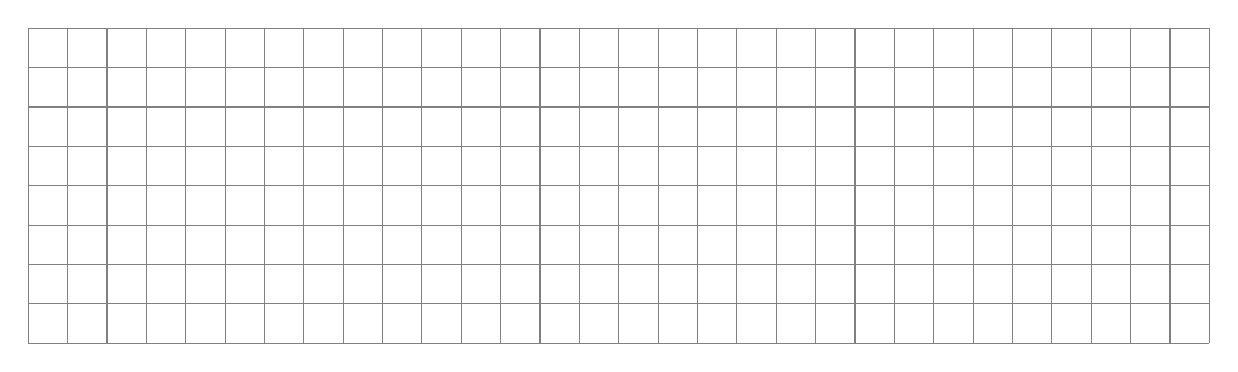
\begin{tikzpicture}
\draw[step=0.5cm,color=gray] (-7,-3) grid (8,\dist);
\end{tikzpicture}
}



%%% Square für größer kleiner Operationen
\def\msquare{\quad\mathord{\scalebox{1.5}[1]{\scalerel*{\Box}{\strut}}} \quad}
